\documentclass[12pt]{article}
\usepackage{graphicx}
\usepackage{subcaption}
\graphicspath{ {images/} }
\usepackage[margin=1in]{geometry}
\usepackage{float}
\title{Propagation of Voltage in a Neuron: The Cable Equation}
\author{Darice Guittet, Elise Niedringhaus, Sarah Liddle}

\begin{document}
\maketitle
\section{Introduction}

Information within the brain is transmitted between neurons largely due to action potentionals, otherwise known as spikes, which are when the voltage in a neuron rapidly rises and falls. These allow communication between brain cells. A.L Hodgkin and A.F. Huxley received a 1963 Nobel Prize for their work regarding this topic, specifically the discovery that individual parts of the axonal membrane behave similarly to a component in an electric circuit. With this knew knowledge, it is now possible to derive equations that represent the voltage propagation in a neuron using formulas similar to those that describe current, resistance, and voltage in an electrical system. This pattern of diffusion along the membrane of neurons by current or voltage is called cable theory, which is what we will be analyzing in this report.

\subsection{Understanding the Model}
The model we are using to understand the propagation of voltage in a neuron can be described by the following partial differential equation:
\begin{equation} \label{1}
\frac{\partial{v(x,t)}}{\partial{t}}=\frac{\partial^2{v(x,t)}}{\partial{x}^2}+f(v(x,t))+J_{ext}(x,t)
\end {equation}
The terms with partial derivatives are from the heat or diffusion equation, mathematically describing the process when molecules move from areas of high concentration to places of low concentration. The $f(v(x,t))$ term accounts for ion channels in a neuron; these open and close to add or decrease from the ions entering the cell based on its current voltage. The $J_{ext}(x,t)$ term accounts for the external voltage that is applied to the neuron. 
\subsubsection{Summary of the Derivation}
This model is derived from equations relating current, voltage, and resistance in an electric circuit, as the work by A.L. Hodgkin and A.F. Huxley demonstrated that parts of the axonal membrane behave similar to a circuit. We will take the membrane to be an infitesimal segment $[x, x+dx]$ with seperate intra- and extracellular voltages and resistances, denoted by either an $i$ or an $e$ in the subscript, respectively. The first step in deriving the model is using Ohm's law to relate current, voltage, and resistance. Note that since we will be examining the voltage in the membrane of a neuron, it is important to examine each of these values inside and outside of the cell; this results in two equations for current. 
\[v_i(x+dx)-v_i(x)=-I_i(x)R_idx\]
\[v_e(x+dx)-v_e(x)=-I_e(x)R_edx\]
If we take these relations, divide by $dx$, and take the limit as $dx\rightarrow 0$ and solve for current, we get the following equations:
\[I_i(x)=-\frac{\partial}{\partial{x}}(\frac{1}{R_i(x)}\frac{\partial{v_i}}{\partial{x}})\]
\[I_e(x)=-\frac{\partial}{\partial{x}}(\frac{1}{R_e(x)}\frac{\partial{v_e}}{\partial{x}})\]
Now, we want to use these two equations to solve for the current per unit length $J_m(x)$, where, for an infitesimal segment, $J_m(x)dx=I_e(x+dx)-I_e(x)=I_i(x+dx)-I_i(x)$. We will divde by $dx$ and take the limit as $dx\rightarrow 0$. This gives the relatioship:
\[J_m(x)=\frac{\partial{I_e}}{\partial{x}}=-\frac{\partial{I_i}}{\partial{x}}\]
We know that the voltage across the cell membrane must be the difference between the intra- and extracellular voltages: $v=v_i=v_e$ and that there is a total current that is constant that will be equal to the sum of the intra- and extracellular current. We will use Ohm's law to write this current in terms of resistance and voltage, rewriting voltages with the relation $v=v_i=v_e$, and plug all these into the sum of currents equation. Since the sum of the currents is constant and we can assume that resistances are constant, we can take the partial derivative with respect to x and get the following relationship between current per unit length $J_m(x)$ and voltage $v$.
\begin{equation} \label{2}
J_m(x)=\frac{\partial}{\partial{x}}(\frac{1}{R(x)}\frac{\partial{v}}{\partial{x}})
\end {equation}
This describes the current passing through the membrane of a neuron, and is also a form of the diffusion equation.\par
Now, we will consider time variables in this model because the model behaves like an RC circuit and have some nonlinear properties of ion channels that act similar to resistors. When the current per unit length has a time variable, it is also the sum of capactive current, outward ionic current, and inward applied current. If we plug this relation into Equation (\ref{2}), we get the following:
\[C\frac{\partial{v(x,t)}}{\partial{t}}=-J_{ION}(v(x,t),t)+\frac{1}{R}\frac{\partial^2{v(x,t)}}{\partial{x}^2}+J_A(x,t)\]
The term $-J_{ION}(v(x,t),t)$ is the outward applied current, can be represented by $f(v(x,t))$, a nonlinear function that controls how voltage leaves or enters the system. The term $J_A(x,t)$ was the inward applied current, and can represent the voltage applied ot the system externally. Now, we will need to change variables in order to get rid of R and C; however, we will still write the final variables as $x$ and $t$ for familiarty. The final model becomes:
\[\frac{\partial{v(x,t)}}{\partial{t}}=\frac{\partial^2{v(x,t)}}{\partial{x}^2}+f(v(x,t))+J_{ext}(x,t)\]

\subsection{Purpose}
In this project, we aim to examine the partial differential equation model of this phenomenon to analyze the propagation of action potentials throughout a neuron. First, we will look at a passive membrane where there is no voltage gradient and ions will leak out of the cell by first solving the stationary solution and then solving the partial differential equation in order to analyze the impulse propagation reaction to various initial voltage inputs. Next, we will analyze a nonlinear model that takes into account that membrane ion channels often have a "two state" nature--meaning... We will examine the traveling wave solutions of this model. Therefore, we aim to have a better understanding of how voltage propagates within under various conditions and inputs.

\section{Passive Membrane}
We consider a passive membrane current with a linear ionic current that obeys Ohm's Law, with the resistance rescaled to unity: $f(v(x,t)) = -v(x,t)$. In addition, we add an external impulse at $x=0$ and $t=0$, formulated as the dirac delta function $\delta(t) \delta(x)$, to examine how the voltage responds. Since axons are much longer than wide, $x$ will range from $-\infty$ to $\infty$. We are also looking for bounded solutions since this is a physical system, therefore we look for solutions such that $\int_{-\infty}^{\infty}|v(x,t)|dx = M < \infty$. The inhomogeneous PDE corresponding to such a system is given by

\begin{equation} \label{pm}
\frac{\partial{v(x,t)}}{\partial{t}}=\frac{\partial^2{v(x,t)}}{\partial{x}^2}-v(x,t)+\delta(t)\delta(x)
\end {equation}

\subsection{Stationary Solutions}
To start, we find the stationary solutions, $v(x,t) = V_0(x)$, satisfying $\frac{\partial{v(x,t)}}{\partial{t}} = 0$ by solving the homogeneous ODE:

\begin{equation} \label{pm_odeH}
\frac{d^2{V_0(x)}}{d{x^2}} - V_0(x) = 0
\end{equation}
The general solution is $V_0(x) = c_1e^{-x} + c_2e^{x}$. However, in order for $V_0$ to be bounded on $(-\infty, \infty)$, $V_0$ = 0:

\subsection{Impulse Response}
We add a stationary input current localized at $x=0$ and find solutions $V_F(x)$ to the resulting inhomogeneous ODE with boundary conditions $\lim_{x\to\infty} V_F(x) = 0$.

\begin{equation} \label{pm_odeN}
\frac{d^2{V_F(x)}}{d{x^2}} - V_F(x) = -\delta(x)
\end{equation}
We compute the Fourier transforms of the ODE to find an algebraic equation for the Fourier transform of the solution $\mathcal{FT}\left\{V_F(x)\right\} = \overline{V_F}(\omega)$, where $\omega$ is the spatial frequency with units $\frac{1}{x}$. Using the fact that $\mathcal{FT}\left\{d_{xx}V_F(x)\right\} = -\omega^2\overline{V_F}(\omega)$ and $ \mathcal{FT}\left\{\delta(x)\right\} = 1$, we get an equation which we can rearrange:

$$  \overline{V_F}(\omega) = \frac{1}{\omega^2+1} $$
From a Fourier transform table (*reference!), we find our solution to be:

$$ V_F(x) = \mathcal{FT}^{-1}\left\{\overline{V_F(\omega)}\right\} =  \frac{1}{2}e^{-|x|} $$

\subsection{Generalizing Solutions}
If we make the change of variable $x = x-x_0$ to Part 2.2, we arrive at the inhomogeneous ODE whose solution is defined to be Green's function for this particular problem. Let $\mathcal{L}\left\{G\right\}$ be the linear operator that is the left-hand side of the equation and $G(x-x_0)$ be Green's function, satisfying the same boundary conditions as above.

\begin{equation} \label{pm_greens}
\mathcal{L}\left\{G\right\} = -\frac{d^2{G(x-x_0)}}{d{x^2}} + G(x-x_0) = \delta(x-x_0)
\end{equation}
$$ G(x-x_0) = \frac{1}{2}e^{-| x-x_0 |} $$
For any external input $f(x)$ and the associated inhomogeneous equation $\mathcal{L}\left\{y\right\} = f(x)$, the solution $y(x)$ can be found as
$$ y(x) = \int_{a}^{b}G(x-x_0)f(x_0)dx_0 $$
This fundamental property of Green's function is due to the \textit{sifting property} of the dirac delta function. 
$$\mathcal{L}\left\{y\right\} = L\int_a^bG(x-x_0)f(x_0)dx_0 = \int_a^b\mathcal{L}\left\{G(x-x_0)\right\}f(x_0)dx_0 = \int_a^b\delta(x-x_0)f(x_0)dx_0 $$
The formula for a stationary solution given an arbitrary stationary input uses Green's function as below.
$$V_A(x) = \int_{-\infty}^{\infty}\frac{1}{2}e^{-|x-x_0|}J_{ext}(x_0)dx_0 $$

\subsection{Green's Function for Time-Dependent Equation}
Returning to the full time-dependent equation (\ref{pm}), we use Fourier transforms to find the solution, $G_{\infty}(x,t)$, Green's function on the infinite cable. This time, the Fourier transform of the PDE results in an inhomogeneous ODE for $\overline{G_{\infty}}(\omega,t)$.

\begin{equation}\label{pm_timeFT}
\frac{d}{dt}\overline{G_{\infty}}(\omega,t) + (\omega^2+1)\overline{G_{\infty}}(\omega,t) = \delta(t) 
\end{equation} 
When $t>0$, $\delta(t) = 0$ so the equation is reduced to a homogeneous ODE. Separation of variables and integration of both sides leads to the homogeneous solution, scaled by a function that is only dependent on $\omega$.

$$ \int\frac{1}{\overline{G_{\infty}}(\omega,t)}d\overline{G_{\infty}}(\omega,t) = -\int(\omega^2 + 1)dt $$
$$ \ln|(\overline{G_{\infty}}(\omega,t)| = -(\omega^2+1)t + c(\omega) $$
 
$$\overline{G_{\infty}}(\omega,t) = c(\omega)e^{-t(\omega^2+1)} $$
To find the value of $c(\omega)$, we examine the solution around $t=0$. Due to $\delta(t)$, there is a discontinuity such that $\overline{G_{\infty}}(\omega,0^-) = 0$ while $\overline{G_{\infty}}(\omega,0^+) = c(\omega)$. We integrate equation (\ref{pm_timeFT}) at a small section around the discontinuity, from $t=(-\epsilon, \epsilon)$, use the fact that $\overline{G_{\infty}}(\omega,\epsilon-) = 0$ since our system starts at $t=0$. 

$$\int_{-\epsilon}^{\epsilon}\frac{d}{dt}\overline{G_{\infty}}(\omega,t)dt + \int_{-\epsilon}^{\epsilon}(\omega^2+1)\overline{G_{\infty}}(\omega,t)dt = \int_{-\epsilon}^{\epsilon}\delta(t)dt $$

$$  \overline{G_{\infty}}(\omega,\epsilon) + \int_{-\epsilon}^{\epsilon}(\omega^2+1)\overline{G_{\infty}}(\omega,t)dt = 1$$
Taking the limit as $\epsilon \to 0$, we find the integral goes to zero and we are left with the constraint.

$$ \lim_{\epsilon\to 0} \overline{G_{\infty}}(\omega,\epsilon)  = \lim_{t\to 0^+}c(\omega)e^{-t(\omega^2+1)}  = 1 $$
Therefore, $c(\omega) = 1$ and our solution for $t>0$ is found to be the inverse Fourier transform.
$$G_{\infty}(\omega,t) = \frac{1}{2\pi}\int_{-\infty}^{\infty}e^{-t(\omega^2+1)}e^{i \omega x)} d\omega = \frac{1}{2\pi}\int_{-\infty}^{\infty}e^{i \omega x-t(\omega^2+1)}d\omega $$
We complete the square for the exponents and recognize the result as a Gaussian integral to find the solution.

$$ G_{\infty}(x,t) = \frac{\mathcal{H}(x,t)}{2\pi}e^{-t-\frac{x^2}{4t}}\int_{-\infty}^{\infty}e^{-t(\omega - \frac{ix}{2t} )^2 }d\omega = \frac{\mathcal{H}(x,t)}{\sqrt{4\pi t}}e^{-t-\frac{x^2}{4t}} $$

\subsubsection{Plots of Green's Function}
We plot Green's function at $t=0$, $t=1$, $t=10$ and $t=100$.

\begin{figure}[H]
    \centering
    \begin{subfigure}[h]{0.4\textwidth}
        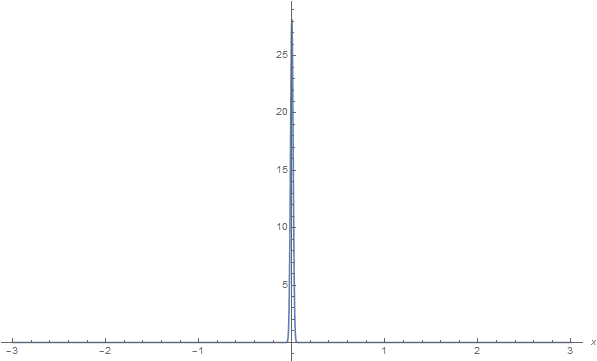
\includegraphics[width=\textwidth]{Part1Plots/t0}
        \caption{$t=0$}
        \label{fig:t0}
    \end{subfigure}
    \begin{subfigure}[h]{0.4\textwidth}
        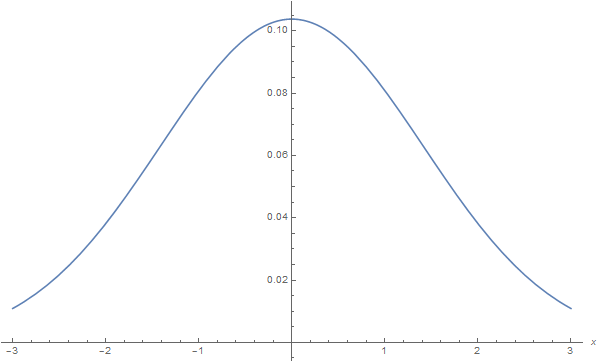
\includegraphics[width=\textwidth]{Part1Plots/t1}
        \caption{$t=1$}
        \label{fig:t1}
    \end{subfigure}
    \begin{subfigure}[h]{0.4\textwidth}
        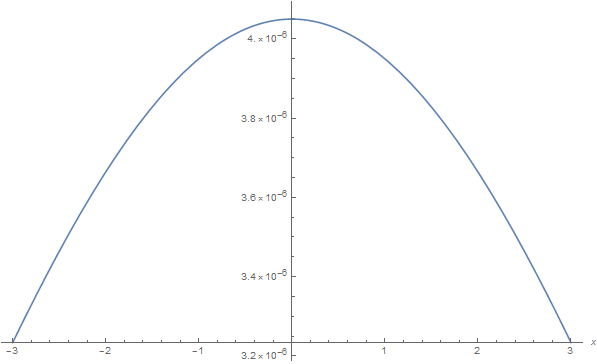
\includegraphics[width=\textwidth]{Part1Plots/t10}
        \caption{$t=10$}
        \label{fig:t10}
    \end{subfigure}
    \begin{subfigure}[h]{0.4\textwidth}
        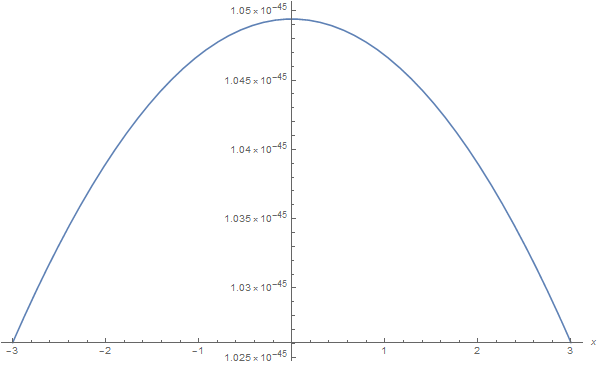
\includegraphics[width=\textwidth]{Part1Plots/t100}
        \caption{$t=100$}
        \label{fig:t100}
    \end{subfigure}
    \caption{Plots of Green's Function at Various Times}\label{fig:timeplots}
\end{figure}

We also plot Green's function at $x=0$, where voltage is monotone decreasing, and $x=2$, where voltage is nonmonotonic, for $t>0$.

\begin{figure}[H]
    \centering
    \begin{subfigure}[h]{0.4\textwidth}
        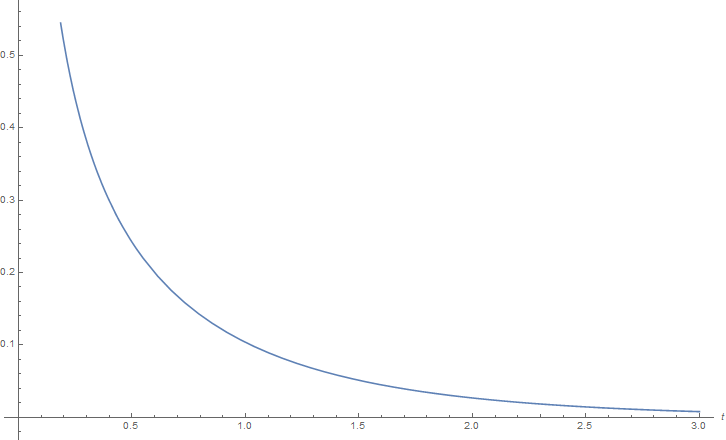
\includegraphics[width=\textwidth]{Part1Plots/x0}
        \caption{$x=0$}
        \label{fig:x0}
    \end{subfigure}
    \begin{subfigure}[h]{0.4\textwidth}
        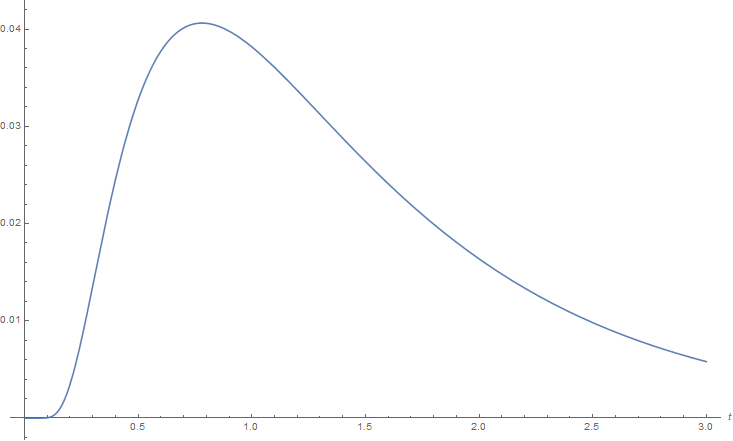
\includegraphics[width=\textwidth]{Part1Plots/x2}
        \caption{$x=2$}
        \label{fig:x2}
    \end{subfigure}

    \caption{Plots of Green's Function at Various Locations}\label{fig:spaceplots}
\end{figure}

The total voltage was computed to be $\int_{-\infty}^{\infty}G_{\infty}(x,t)dx = e^{-t}, t>0$ and it is monotone decreasing.

\begin{figure}[H]
	\centering
	\begin{subfigure}[h]{0.8\textwidth}
        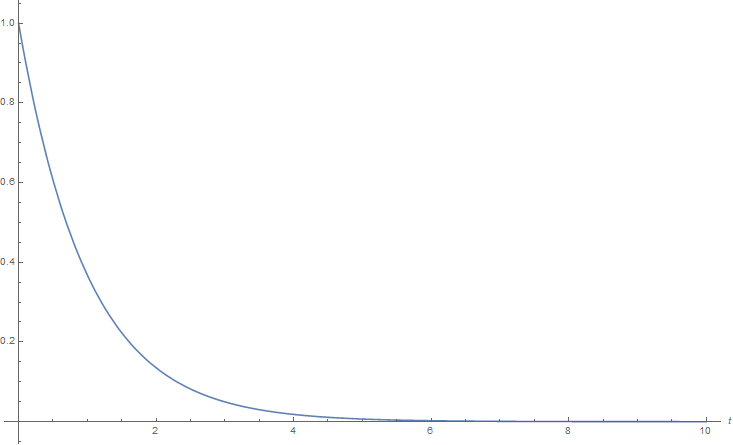
\includegraphics[width=\textwidth]{Part1Plots/g}
    \end{subfigure}
    \caption{Total Voltage} \label{fig:totalvoltage}
\end{figure}
   	
   	
\subsection{Generalizing Solutions}
Using Green's function found above, the formula for a generalized solution given arbitrary spatiotemporal input $J_{ext}(x,t)$ is

$$ \int_{-\infty}^{\infty}\int_{-\infty}^{\infty}G_{\infty}(x-x_0,t-t_0)J_{ext}(x_0,t_0)dx_0dt_0 $$

\pagebreak

\subsubsection{Example Function 1}
For $J_{1}(x,t) = [\delta(x-1)+\delta(x+1)]\delta(t)$, with a starting momentary impulse at $x=1$ and $x=-1$ , the solution is found and plotted below.

$$ v_1(x,t) = \frac{\mathcal{H}(t)}{2\sqrt{\pi t}}(1+e^{\frac{x}{t}})e^{-t-\frac{(1+x)^2}{4t}} $$

\begin{figure}[H]
	\centering
	\begin{subfigure}[h]{0.8\textwidth}
        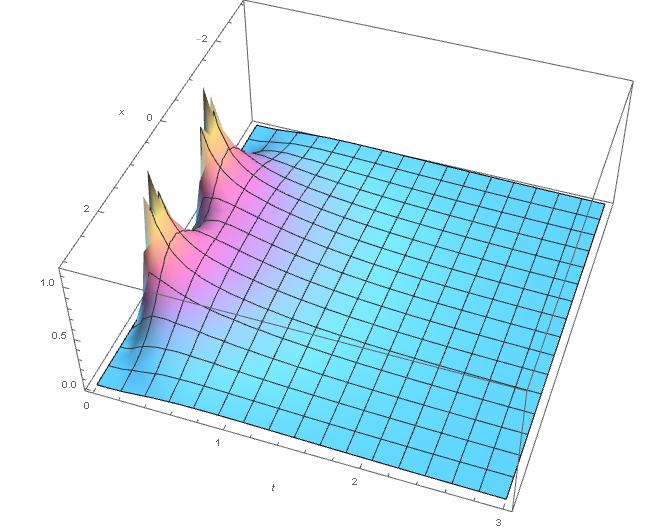
\includegraphics[width=\textwidth]{Part1Plots/plot1}
    \end{subfigure}
    \caption{Plot of $v_1(x,t)$ with $J_{1}(x,t)=[\delta(x-1)+\delta(x+1)]\delta(t)$} \label{fig:jext1}
\end{figure}

\pagebreak
\subsubsection{Example Function 2}
For $J_{2}(x,t) = 1$, the solution and plot is:
$$ v_2(x,t) = 1 $$

\begin{figure}[H]
	\centering
	\begin{subfigure}[h]{0.8\textwidth}
        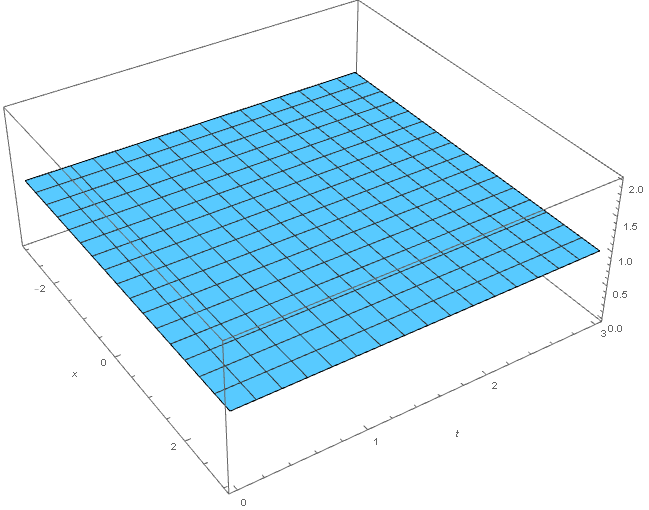
\includegraphics[width=\textwidth]{Part1Plots/plot2}
    \end{subfigure}
    \caption{Plot of $v_2(x,t)$ with $J_{2}(x,t)=1$} \label{fig:jext2}
\end{figure}


\pagebreak
\subsubsection{Example Function 3}
For $J_{3}(x,t) = sin(x)$, the solution and plot is:
$$ v_3{x,t} = \frac{sin(x)}{2} $$

\begin{figure}[H]
	\centering
	\begin{subfigure}[h]{0.8\textwidth}
        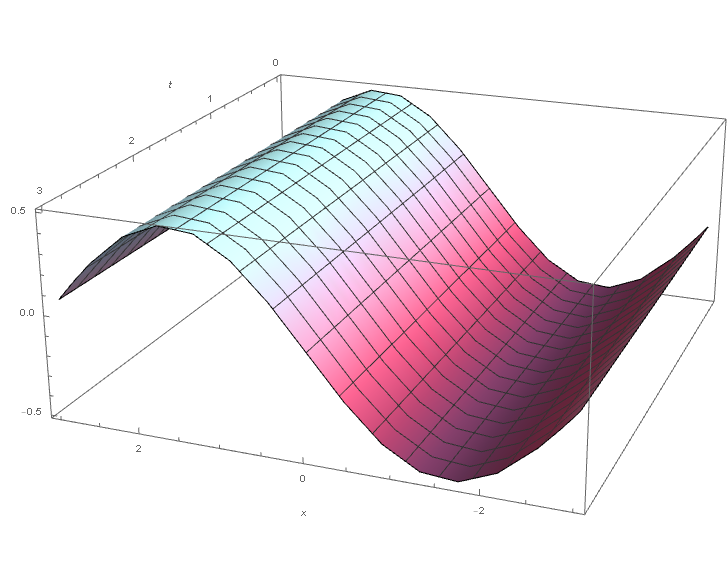
\includegraphics[width=\textwidth]{Part1Plots/plot3}
    \end{subfigure}
    \caption{Plot of $v_{3}(x,t)$ with $ J_3(x,t) = \frac{sin(x)}{2} $ } \label{fig:jext3}
\end{figure}

\pagebreak

\section{Numerical Solutions}
After analytically solving the voltage equation, we also found numerical solutions. In order to numerically solve for this partial differential equation, we must first discretize both partial derivatives. For this problem, discretization is the process of using Taylor series to approximate the first time derivative of the voltage function in terms of the point we will approximate and the known point one time step before it, like so:
\[\frac{\partial{v(x,t)}}{\partial{t}}=\frac{v^{j+1}_i-v^j_i}{\Delta{t}}+O(\Delta{t})\]
In this equation, $v^j_i$ represents the point at $x=x_i$ and $t=t_j$ and $O(\Delta{t})$ represents the order of the error of this approximation, meaning that the error is a function of the size of the timestep.
Using the same approach, we will use Taylor series to write the second x derivative of the voltage function in terms of three known points, like so:
\[\frac{\partial^2{v(x,t)}}{\partial{x}^2}=\frac{v^{j}_{i+1}-2v^j_i+v^j_{i-1}}{(\Delta{x})^2}+O((\Delta{x})^2)\]
Using these two formulas and putting these into our original PDE gives:
\[\frac{v^{j+1}_i-v^j_i}{\Delta{t}}=\frac{v^{j}_{i+1}-2v^j_i+v^j_{i-1}}{(\Delta{x})^2}-v^j_i+J_{ext}(x,t)\]
Finally, we can algebraically solve this equation for $v^{j+1}_i$, in terms of values that are known. Therefore, going timestep by timestep starting from the initial condition, this question can be used to solve numerically for the entire subset of the neuron we're examining. Note that I have removed the $J_{ext}(x,t)$ from this equation
\begin{equation} \label{*}
v^{j+1}_i=\frac{\Delta{t}}{(\Delta{x})^2}(v^{j}_{i+1}+v^{j}_{i-1})+(1-\frac{\Delta{t}(2+(\Delta{x})^2)}{(\Delta{x})^2})v^{j}_{i}+\Delta{t}*J_{ext}(x,t)
\end {equation}
However, looking at the $v^{j}_{i}$ term in this equation, it can be seen that if $\frac{\Delta{t}(2+(\Delta{x})^2)}{(\Delta{x})^2}>1$ then this approximation is unstable and will not converge. Therefore, in order for this method of finite difference approximation to converge, $\Delta{t}$ must be much smaller than $\Delta{x}$ 
When using equation (\ref{*}) to approximate this solution numerically, we will be using $J_{ext}(x,t)=10e^{-25x^2}\delta{(t)}$. However, instead of simulating the function $\delta{(t})$, we will remove $J_{ext}(x,t)$ from the function representing the numerical function and use it as the initial condtion, making $v(x,0)=10e^{-25x^2}$. The boundary conditions will be zero everywhere else. Since we cannot approximate an infinite interval of x and t, we will instead look at the region from $[-10,10]$ for x and $[0,50]$ for t. 
First, using the given $\Delta{t}=0.1$ and $\Delta{x}=0.1$, we can see the the approximation does not converge to a solution, as predicted, and that it is unstable. 
\begin{figure}[H]
  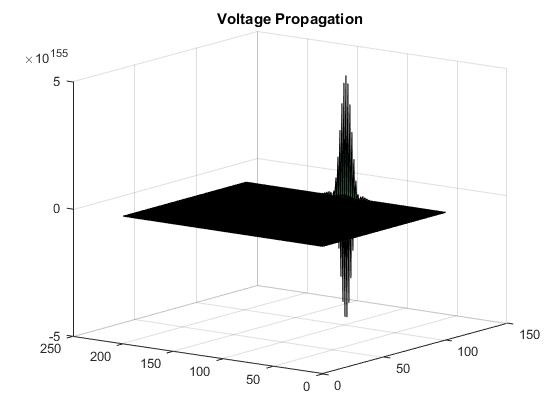
\includegraphics[width=\linewidth]{plot1.jpg}
  \caption{Plot of Unstable Numerical Approximation}
  \label{fig:sketch1}
\end{figure}
In this figure, we had to shorten the total time to 10 seconds because by time fifty, the instability casued parts of the solutions to approach infinity, so Matlab was not able to plot it reasonably. One can see in this plot that as time increases, the voltage increases exponentially higher than it began. \par
Next, when we change $\Delta{t}$ to 0.001 the meet the conditions for stability of this approximation, we can see that the approximation closely resembles our analytic solution to this partial differential equation.
\begin{figure}[H]
  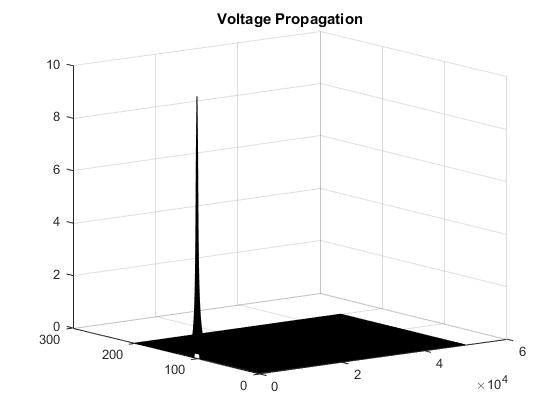
\includegraphics[width=\linewidth]{Plot2.jpg}
  \caption{Plot of Stable Numerical Approximation}
  \label{fig:sketch2}
\end{figure}
As one can see, this plot is matches closely to the analytical solution. It shows the spike of voltage at $t=0$ and $x=0$ and demonstrates how that voltage propagates throughout the neuron, approaching zero as time and x increases. \par
In order to make the propagation more apparent, I included the graph below, where each line indicates a different time step:
\begin{figure}[H]
  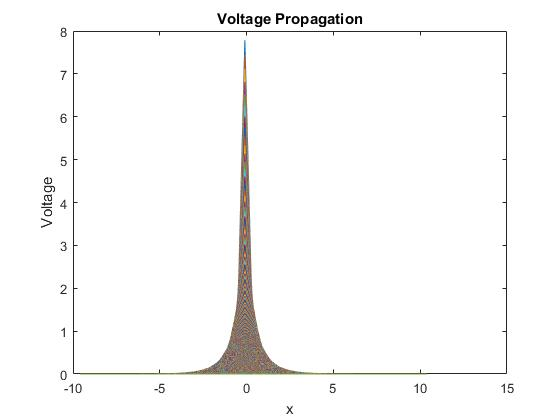
\includegraphics[width=\linewidth]{othergraph1.jpg}
  \caption{Plot of Stable Numerical Approximation}
  \label{fig:sketch2}
\end{figure}
Next, I displayed a plot of the voltages for only the times 25-50 seconds, to show the scaling on the remaining values. Although they appear to all be zero in the initial graph, they are nonzero and diminishing as one would expect with ions leaking out of the cell, as is the case in this scenario.
\begin{figure}[H]
  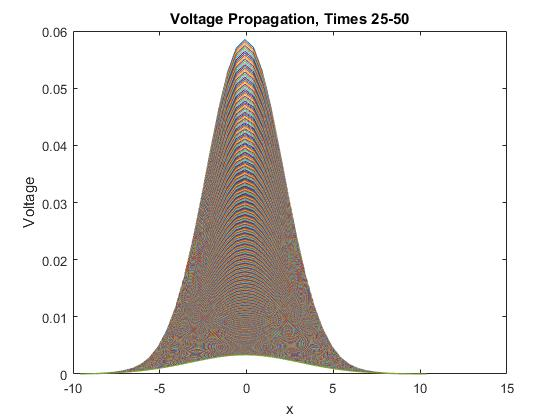
\includegraphics[width=\linewidth]{othergraph2.jpg}
  \caption{Plot of Stable Numerical Approximation, Times 25-50}
  \label{fig:sketch2}
\end{figure}

\section{The Bistable and Traveling Wave Solution}

\subsection{Numerical Solutions: Two-State Ion Channels}
After analytically solving te traveling wave solutions of the voltage equation, we found numerical solutions as well. In this case, the equation we examined was:
\[\frac{\partial{v(x,t)}}{\partial{t}}=\frac{\partial^2{v(x,t)}}{\partial{x}^2}-v(x,t)+H(v(x,t)-\theta)+J_{ext}(x,t)\]
Though the term $J_{ext}(x,t)$ was not specified, I will used $J_{ext}(x,t)=10e^{25x^2}\delta{t}$. This is the same $J_{ext}(x,t)$ used in numerically solving the passive membrane solution, and it can be removed from the equation itself and substituted into the initial condition. It mimics the scenario of a large spike of voltage initially applied to the neuron at $x=0$ and $t=0$, while remaining almost zero for all other $x$ at $t=0$. Also, though there are infinite boundaries for both $x$ and $t$, we will again only look at the region from $[-10,10]$ for x and $[0,50]$ for t in order to numerically solve this system.  Similar to the numerical solutions of the passive membrane, we will solve the system numerically by discretizing both partial derivatives using Taylor series, plugging these approximations back into the original partial differential equation, and solving for $v^{j+1}_i$. This gives the equation:
\begin{equation} \label{**}
v^{j+1}_i=\frac{\Delta{t}}{(\Delta{x})^2}(v^{j}_{i+1}+v^{j}_{i-1})+(1-\frac{\Delta{t}(2+(\Delta{x})^2)}{(\Delta{x})^2})v^{j}_{i}+\Delta{t}*H(v^j_i-\theta)
\end {equation}
This equation requires the same stability condition as the numerical approximation for the passive membrane solution. If $\frac{\Delta{t}(2+(\Delta{x})^2)}{(\Delta{x})^2}>1$ then this approximation is unstable and will not converge. Therefore, $\Delta{t}$ must be much smaller than $\Delta{x}$. This instability is demonstrated when we use the given values of $\Delta{x}=0.1$ and $\Delta{t}=0.1$. 
\begin{figure}[H]
  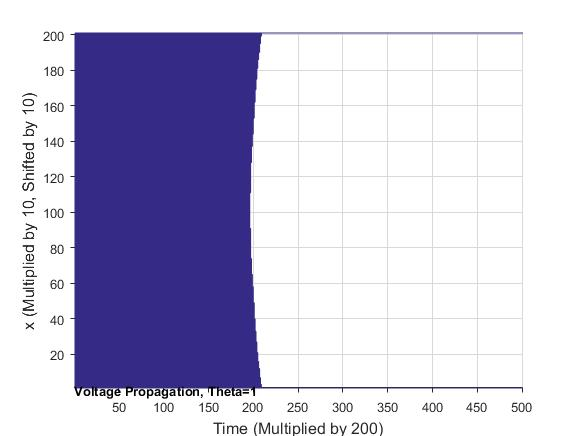
\includegraphics[width=\linewidth]{badplot3.jpg}
  \caption{Plot of Unstable Numerical Approximation, Two-State Ion Channel Solution}
  \label{fig:sketch3}
\end{figure}
Matlab was unable to plot this completely, because the divergance caused some of the points to not be able to compute. Therefore, for the rest of the problem, we will make $\Delta{x}=0.5$ and $\Delta{t}=0.005$. Next, we will produce plots of numerical solutions with three different values of $\theta$. The values we examined were $\theta=1$, $\theta=0.5$, $\theta=0.1$. 
\begin{figure}[H]
  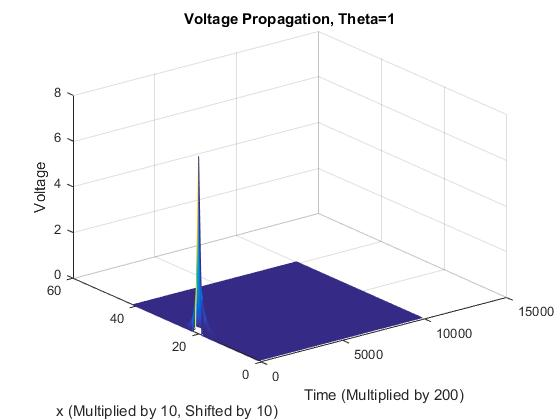
\includegraphics[width=\linewidth]{thetaone.jpg}
  \caption{Plot of Stable Numerical Approximation, Two-State Ion Channel Solution, $\theta=1$}
  \label{fig:sketch4}
\end{figure}
With this value of $\theta$ the plot doesn't look much different from the plots in the passive membrane solution. This is because when $\theta$ is large, not many of values of voltage, $v(x,t)$ will be greater than $\theta$ so the Heaviside function will be zero for most of the soltuion. Since this value of $\theta$ doesn't produce a traveling wave, we cannot numerically calculate the speed of the wave. 
\begin{figure}[H]
  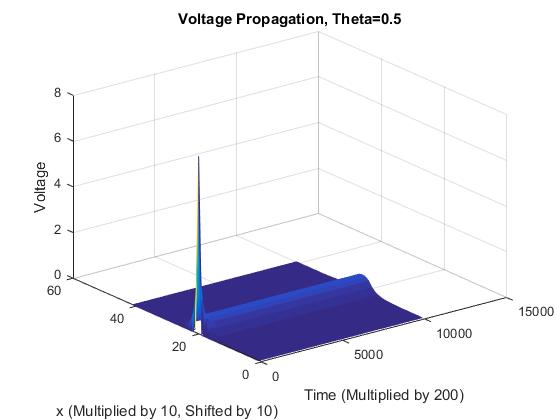
\includegraphics[width=\linewidth]{thetatwo.jpg}
  \caption{Plot of Stable Numerical Approximation, Two-State Ion Channel Solution, $\theta=0.5$}
  \label{fig:sketch5}
\end{figure}
With this value of $\theta$, there is a single wave of voltage, but its speed is zero. By exmining hte graph, one can see that it converges to relatively constant position as time increases.This is verified for plugging in $\theta=1$ to the analytical equation for wave speed as a function of $\theta$ we found earlier in the report. As time increases, the solution converges to a uniform wave that doesn't change shape and remains stationary throughout time.
\begin{figure}[H]
  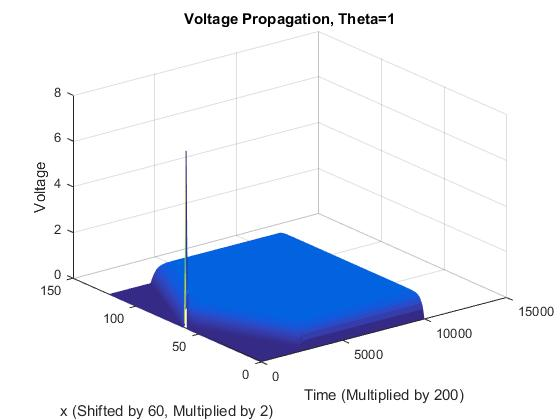
\includegraphics[width=\linewidth]{thetathree.jpg}
  \caption{Plot of Stable Numerical Approximation, Two-State Ion Channel Solution, $\theta=0.1$}
  \label{fig:sketch6}
\end{figure}
We found that for this value of $\theta$, the traveling wave front was better depicted with a wider range of x values, so x will go between $[-30,30]$ in this plot. One can see that initially, the wave is spreading from the center $x=0$ to the edges of the boundary. In an infinite boundary, this wave would spread throughout the entire neuron. 
\subsubsection{Periodically Varying Threshold}
Now, we will find numerical solutions for a periodically varying threshold. This will be represented in our model by substituting in the following for $f(v(x,t))$:
\[f(v,x)=-v+H(v-\theta(1+0.5\cos(x)))\]
However, since we will want to examine the effects of different coefficients in front of the $\cos(x)$ term, I will label this coefficient $C$. The same steps are applied in order to find numerical solutions, where we discretize the parital derivatives and solve in terms of the value at the next timestep. Since this $f(v(x,t))$ is similar to the one in the previous model that we solved numerically for, the numerical approximation will look similar. It is shown below. 
\begin{equation} \label{***}
v^{j+1}_i=\frac{\Delta{t}}{(\Delta{x})^2}(v^{j}_{i+1}+v^{j}_{i-1})+(1-\frac{\Delta{t}(2+(\Delta{x})^2)}{(\Delta{x})^2})v^{j}_{i}+\Delta{t}*H(v^j_i-\theta(1+C\cos(x)))
\end {equation}
In order to analyze the numerical solutions, we used the three different values of $\theta$ from the numerical solution of the previous model, $\theta=1$, $\theta=0.5$, and $\theta=0.1$. For each of these three $\theta$ values, we used four different values of $C$, the constant preceding the $\cos(x)$ term. The first of which was the given value, 0.5, and the rest were $C=20$, $C=2$, and $C=-1$. All of these plots are shown below, grouped together by $\theta$ value
\begin{figure}[H]
  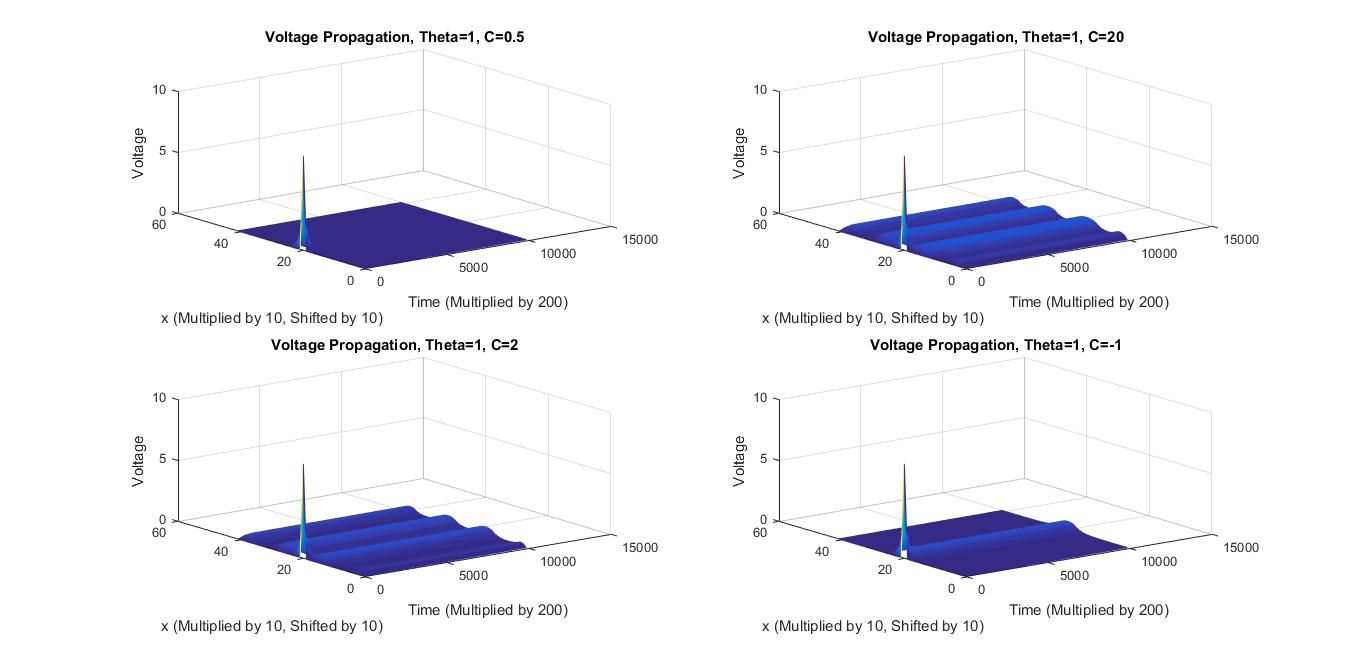
\includegraphics[width=\linewidth]{thetaone3.jpg}
  \caption{Plots of Periodically Varying Threshold, $\theta=1$}
  \label{fig:sketch7}
\end{figure}
\begin{figure}[H]
  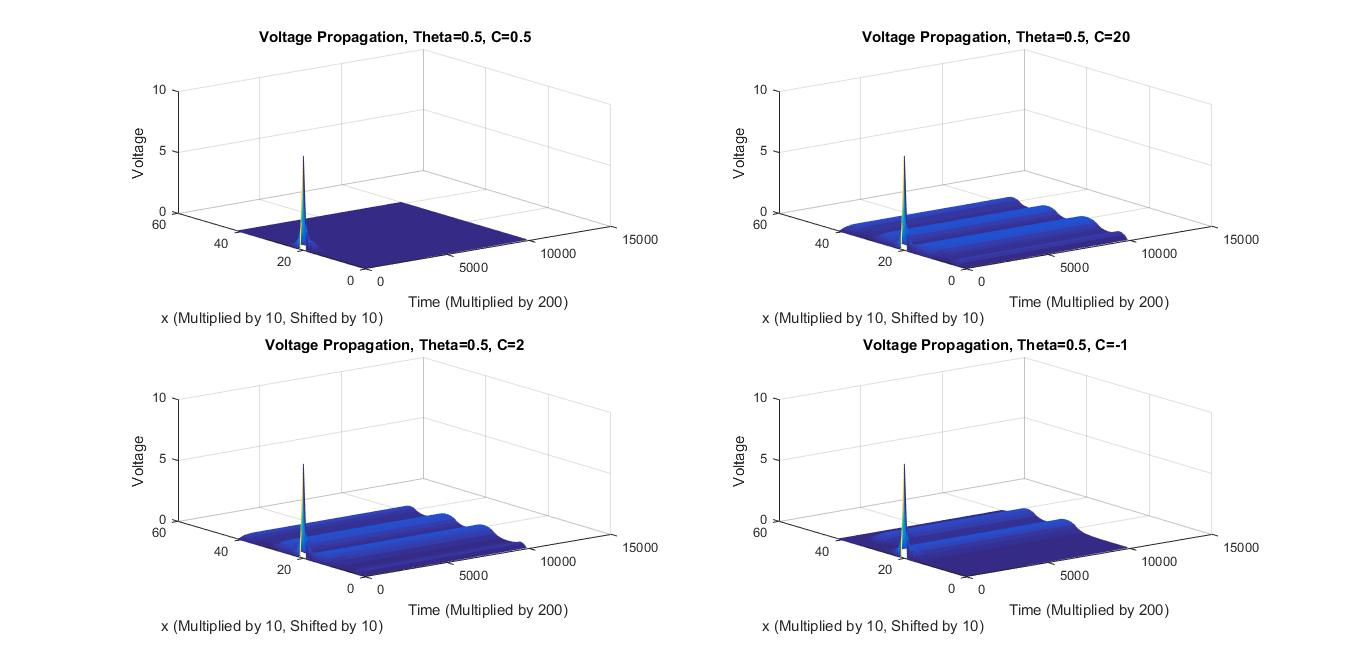
\includegraphics[width=\linewidth]{thetatwo3.jpg}
  \caption{Plots of Periodically Varying Threshold, $\theta=0.5$}
  \label{fig:sketch8}
\end{figure}
\begin{figure}[H]
  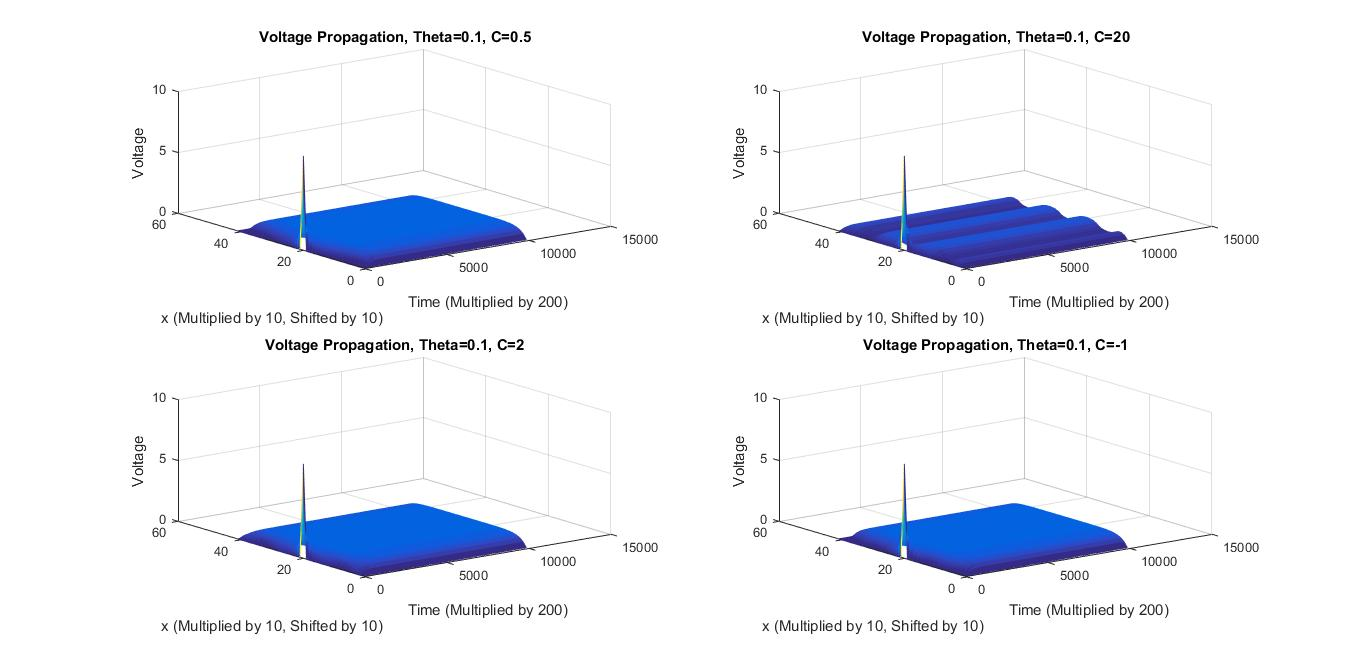
\includegraphics[width=\linewidth]{thetathree3.jpg}
  \caption{Plots of Periodically Varying Threshold, $\theta=0.1$}
  \label{fig:sketch9}
\end{figure}
It seems that if the constant $C$ is too small not much changes from the prior solution, with $f(v(x,t))=H(v^j_i-\theta)$. This is because it causes the constant $C$ determines how much the total alue of $\theta(1+C\cos(x))$ can vary. If it has larger maginitude, it will be less likely that the variable in the Heaviside function (in this case $v_i^j$) will be larger than it when $\cos(x)=1$ or close to it, and when $\cos(x)=0$ or near this area, it is more likely that $v_i^j$ will be larger, so the value of the Heavisde function will be one. However, if $C$ is small, then these periodic fluctuations due to the cosine term will be relatively insignificant. Next, I will examine if drastically increasing the value of $C$ will have a significant effect on the same $\theta$.
\begin{figure}[H]
  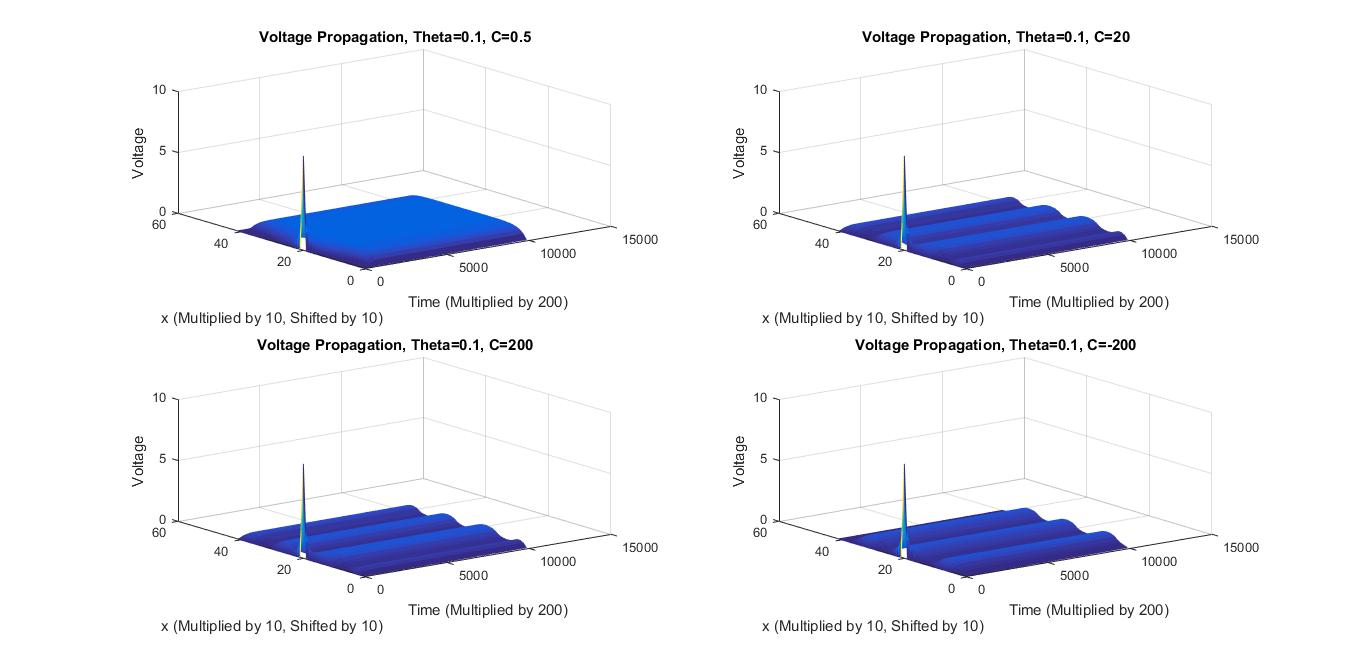
\includegraphics[width=\linewidth]{plotsomething.jpg}
  \caption{Varying $C$, $\theta=0.1$}
  \label{fig:sketch10}
\end{figure}
It appears that once $C$ is above a certain threshold, the magnitude of $C$ will not have a large effect on the waves. This makes sense because most voltage values in the orginal equation are close to zero, so they will only be larger than $\theta(1+C\cos(x))$ when $\cos(x)$ is close to zero anyway, which will result in roughly the same points being affected by the Heaviside function, no matter the magnitude of $C$. Therefore, the average speed of the front is not affected if the constant is increased drastically. 

\section{Conclusions}
In this report, we have analyzed variations of the cable equation in order to better understand the ways in which voltage can propagate throughout a neuron. After summarizing the derivation of the model, we analyzed an action potential imposed on a neuron that is experiencing ions leaking out of the cell. This was our passive membrane solution, and our models confirmed what one might expect--a large spike of voltage initially that is quickly dispersed throughout the neuron and diminished through leaking ions until the voltage goes back to zero, or its original voltage state. \par
In addition, we also analyzed a situation where the neuron has a bistable membrane which allowed us to analyze traveling waves in a solution. Our results verified our expectations, demonstrating how voltage in a neuron can propogate similar to waves approaching shore, rather than just spreading out. We were also able to numerically approximate these solutions in order to verify our results, and numerically approximate systems with more complex functions representing the opening and closing of ion channels that might be more difficult to solve analytically. Through our findings, we were able to expand our knowledge of partial differential equations and Fourier transforms by examining the cable equation and modeling voltage in a neuron. 





















\end{document}